% $Id: ESMF_inframethodoverview.tex,v 1.29 2010/05/15 12:49:16 oehmke Exp $

\section{Overview of Distributed Data Methods}

FieldBundles, Fields, and Arrays all have versions of the following
data communication methods.  In these objects, data is communicated 
between DEs.  Depending on the underlying communication 
mechanism, this may translate within the framework to a data 
copy, an MPI call, or something else.  
The ESMF goal of providing
performance portability means the framework will in the future
attempt to select the
fastest communication strategy on each hardware platform transparently 
to the user code.  (The current implementation uses MPI for communication.)

Communication patterns, meaning exactly which bytes need to be copied 
or sent from one PET to another to perform the requested operation,
can be precomputed during an initialization phase and then later 
executed repeatedly.
There is a common object handle, an {\tt ESMF\_RouteHandle}, which
identifies these stored communication patterns. 
Only the {\tt ESMF\_RouteHandle} and the source and destination 
data pointers must be supplied at runtime to minimize execution overhead.

\subsection{Higher Level Functions}
The following three methods are intended to map closely to 
needs of applications programs.  They represent higher level
communications and are described in more detail in the following
sections.  They are:

\begin{itemize}

\item {\bf Halo}
Update ghost-cell or halo regions at the boundaries
of a local data decomposition.
\item {\bf Regrid}
Transform data from one Grid to another, performing
any necessary data interpolation.
\item {\bf Redist}
Copy data associated with a single Grid from
one decomposition to another.  No data interpolation is necessary.

\end{itemize}

\subsection{Lower Level Functions}
The following methods correspond closely to the lower level
MPI communications primitives.  They are:

\begin{itemize}

\item {\bf Gather}
Reassembling data which is decomposed over a set of DEs into a single
block of data on one DE.
\item {\bf AllGather}
Reassembling data which is decomposed over a set of DEs into multiple
copies of a single block of data, one copy per original DE.
\item {\bf Scatter}
Spreading an undecomposed block of data on one DE over a set of DEs,
decomposing that single block into smaller subsets of data, one
data decomposition per DE.
\item {\bf AlltoAll}
Spreading an undecomposed block of data from multiple DEs onto
each of the other DEs in the set, resulting in a set of multiple decomposed 
data blocks per DE, one from each of the original source DEs.
\item {\bf Broadcast}
Spreading an undecomposed block of data from one DE onto all other
DEs, where the resulting data is still undecomposed and simply
copied to all other DEs.
\item {\bf Reduction}
Computing a single data value, e.g. the data maximum, minimum, sum, etc
from a group of decomposed data blocks across a set of DEs, where the
result is delivered to a single DE.
\item {\bf AllReduce}
Computing a single data value, e.g. the data maximum, minimum, sum, etc
from a group of decomposed data blocks across a set of DEs, where the
result is delivered to all DEs in the set.

\end{itemize}

\subsection{Common Options}
\label{sec:routeoptions}

ESMF will select an appropriate default for the
internal communication strategy for executing the communications.  
However, additional control is available
to the user by specifying the following route options.
(For more details on exactly what changes with the various options,
see Section \ref{sec:routeimpl}.)

\subsection{Design and Implementation Notes}
\label{sec:routeimpl}

\begin{enumerate}

\item

There is an internal {\tt ESMC\_Route} class which supports the 
distributed communication methods.  There are 4 additional internal-only
classes which support {\tt ESMC\_Route}: {\tt ESMC\_AxisIndex}, 
{\tt ESMC\_XPacket}, {\tt ESMC\_CommTable}, and {\tt ESMC\_RTable};
and a public {\tt ESMF\_RouteHandle} class which is what the user 
sets and gets.  The implementation is in C++, with interfaces in Fortran 90.

The general communication strategy is that each
DE computes its own communication information independently,
in parallel, and adds entries to a per-PET route table
which contains all needed sends and receives (or gets and puts) 
stored in terms relative to itself.  (Implementation note: this
code will need to be made thread-safe if multiple threads are
trying to add information to the same route table.)

AxisIndex is a small helper class which contains an index minimum
and maximum for each dimension and is used to describe an n-dimensional
hypercube of information in index space.  These are associated with 
logically rectangular grids and local data arrays.  
There are usually multiple instances of them, for example the local
data chunk, and the overall global index-space grid this data is
a subset of.  Within each of the local or global categories, there are
also multiple instances to describe the allocated space, the total area,
the computational area, and the exclusive area.  See Figure \ref{fig:halo}
for the definitions of each of these regions.
%%%
%%\begin{description}
%%\item [allocated space] all memory associated with this data block
%%\item [total area] subset of allocated area which includes halo regions 
%%but not unused space allocated simply for padding or alignment reasons
%%\item [computational area] subset of total area which includes all data 
%%which is computed, excludes halo regions 
%%\item [exclusive area] subset of computational area data which is not 
%%read for halo updates
%%\end{description}
%%%
(Implementation note: the allocated space is only partially implemented
internally and has no external user API yet.)

An Exchange Packet (XPacket) describes groups of memory addresses
which constitute an n-dimensional hypercube of data.
Each XPacket has an offset from a base address, 
a contiguous run length, 
a stride (or number of items to skip) per dimension,
and a repeat count per dimension. 
See Figure \ref{fig:xpacketbasic} for a diagram of how the XPacket
describes memory.
The actual unit size stored in an XPacket is an item count, 
so before using an XPacket to address bytes of memory
the item size must be known and the
counts multiplied by the number of bytes per item.  This allows
the same XPacket to describe different data types which have the
same memory layout, for example 4 byte integers and 8 byte reals/doubles.
The XPacket methods include basic set/get, how to turn
a list of AxisIndex objects into an XPacket, compute a local XPacket from one
in global (undecomposed grid) space, and a method to compute the intersection
of 2 XPackets and produce a 3rd XPacket describing that region.  

\begin{center}
\begin{figure}
\scalebox{0.9}{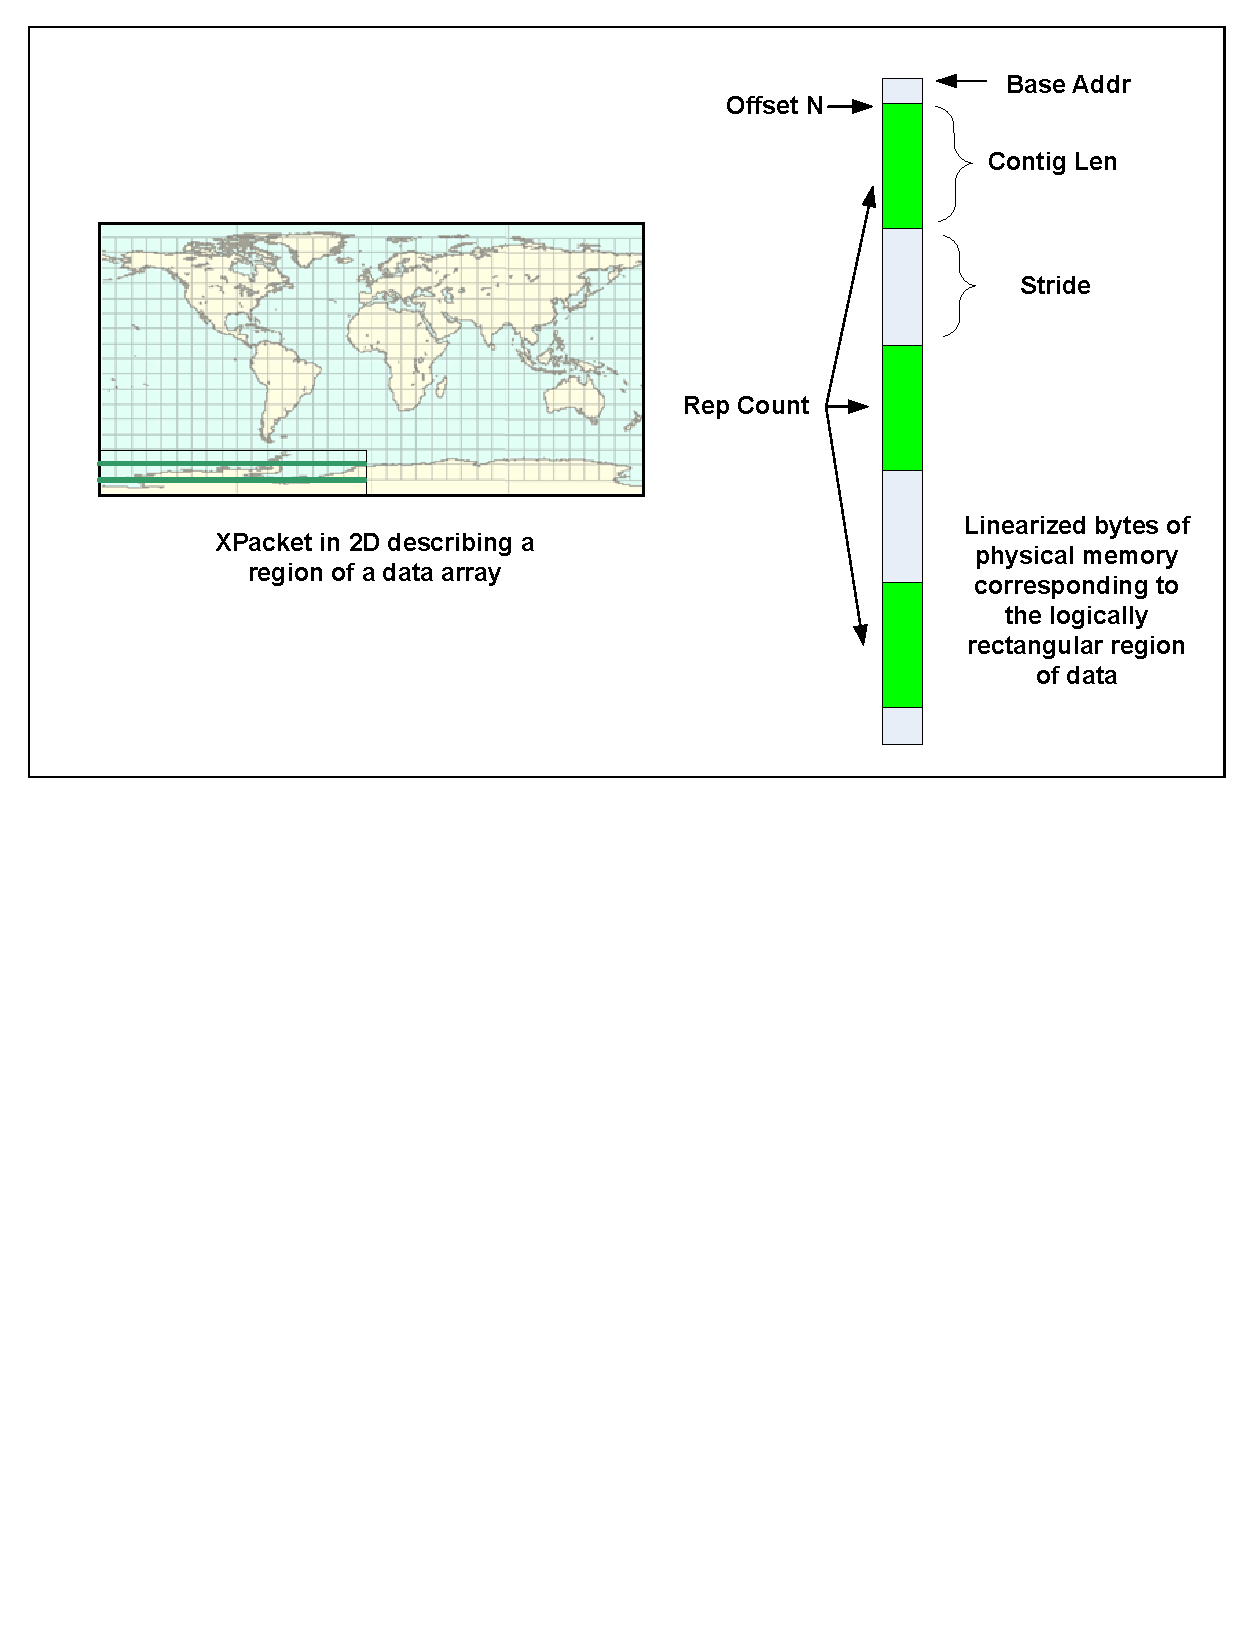
\includegraphics{Basic_xpacket}}
\caption{How an Exchange Packet (XPacket) describes the memory
layout for a rectangular hypercube of data.}
\label{fig:xpacketbasic}
\end{figure}
\end{center}

The Communication Table (CommTable) class encapsulates which other PETs this
PET needs to talk to, and in what order.  There are create and destroy
methods, methods to set that a PET has data either to
send or receive, and query routines that return an answer
to the question 'which PET should I exchange data with next'.  

The Route Table (RTable) class contains a list of
XPackets to be sent and received from other PETs.
It has create/destroy methods, methods to add XPackets to the list for 
each PET, and methods to retrieve the XPackets from any list.

The top level class is a Route.  A Route object contains a send RTable, 
a recv RTable, a CommTable, and a pointer to a Virtual Machine.   
The VM must include all PETs which are participating
in this communication.
The Route methods
include create/destroy, setting a send or recv XPacket
for a particular PET,
and some higher level functions specific to each
type of communication, for example RoutePrecomputeHalo
or RoutePrecomputeRedist.  These latter functions
are where the XPackets are actually computed and added to
the Route table.  Each DE computes its own set of intersections,
either source or destination, and fills its own corresponding PET table.
The Route methods also include a RouteRun method which executes the code
which actually traverses the table and sends the information between PETs.

A RouteHandle class is a small helper class which is returned through
the public API to the user when a Route is created, and passed back in
through the API to select which precomputed Route is to be executed.
A RouteHandle contains a handle type and a pointer to a Route object.
In addition, for use only by the Regrid code, there is an additional Route
pointer and a TransformValues pointer.  (TransformValues is an internal
class only used by the Regridding code.)  If the RouteHandle describes the
Route for a FieldBundle, then the RouteHandle can contain a list of Routes,
one for each Field in the FieldBundle, and for Regrid use, a list of additional
Routes instead of a single Route.  There is also a flag to indicate whether
a single Route is applicable to all Fields in a FieldBundle or whether there
are multiple Routes.
The RouteHandle methods are fairly basic; mostly accessor methods
for getting and setting values.


\item

While intended for any distributed data communication method,
the current implementation only builds a Route object for
the halo, redist, and regrid methods.  Scatter, Gather,
AllGather, and AlltoAll 
should have the option of building a Route for operations
which are executed repeatedly.  This should only require
writing a Precompute method for each one; the existing 
RouteRun can be invoked for these operations.
(This is a lack-of-implementation-time issue, not a design
or architecture issue.)

\item

The original design included automatic detection of different
Routes and internal caching, so the user API did not have to
include a RouteHandle object to identify which Route was
being invoked.  However, users requested that the framework
not cache and that explicit RouteHandle arguments be created
and required to invoke the distributed data methods.
Nothing prevents this code from being revived from the CVS
repository and reinstated in the system, should automatic
caching be desired by future users.

\item

The current distributed methods have 2 related but distinct
interfaces which differ in what information they require
and whether they use RouteHandles:

\begin{enumerate}
\item[Precompute/Run/Release]
This is the most frequently used interface set.
It contains 3 distinct phases: precomputing which bytes must
be moved, actually executing the communications operation,
and releasing the stored information.  This is intended for
any communication pattern which will be executed more than once.
\item[All-in-One]
For a communication which will only be executed once, or in
any situation in which the user does not want to save a RouteHandle,
there are interfaces which do not have RouteHandles as part of
the argument list.  Internally the code computes a Route,
executes it, and releases the resources before returning.
\end{enumerate}

\item

The current CommTable code executes one very specific communication
strategy based on input from a user who did extensive timing
measurements on several different hardware platforms.  Rather than
broadcasting all data at once asychronously, it selects combinations
of pairs of processors and has them execute a SendRecv operation, which
does both a data send and a data receive in a single call.
At each step in the execution, different pairs of processors
exchange data until all pair combinations have been selected.

The table itself must be a power of 2 in size; the number of
PETs is rounded up to the next power of 2 and then all entries
for PETs larger than the actual number are marked as no-ops.

There are many alternative execution strategies, including a
completely asynchronous execution, in numeric PET order, without
computing processor pairs.  Also single-direction communications 
are possible (only the Send XPackets are processed, or only
the Receive XPackets) in either a synchronous or asynchronous mode.  
This would not require any changes to the XPacket or RTable classes,
but would require writing a set of alternative RouteRun methods.

\item

The current RouteRun routine has many possible performance options for how
to make the tradeoff between time spent packing disjoint memory
blocks into a single buffer to minimize the number of sends,
verses simply sending the contiguous blocks without the pack overhead.
The tradeoffs are not expected to be the same on all systems;
hardware latency verses bandwith characteristics will differ,
plus the underlying communication software (MPI, shared memory, etc)
will change the performance.  Also the size of the data blocks
to be sent, the amount of contiguity, and limits on the number 
of outstanding communication buffers all affect what options are best.

The {\tt ESMF\_RouteOptions} are listed in \ref{sec:routeoptions}; 
the following description contains more implementation detail 
about what each of the options
controls inside the execution of a Route.  Note that the options
do not affect the creation of a Route, nor any of the Precompute
code, and can optionally be changed each time the Route is run.

Packing options:
\begin{enumerate}
\item[By Buffer]
If multiple memory addresses are provided to RouteRun (from
bundle-level communications, for example), then this option
packs data across all buffers/blocks as specified by the other
packing flags before sending or receiving.
Note: unlike the other packing flags, this is handled in the
code at a higher level by either passing down multiple addresses
into the route run routine or not.  If multiple addresses are
passed into the run routine, they will be packed.  The "no-packing"
option at this level would be identical to looping at the outermost
level in the RouteRun code and therefore there is no disadvantage
to calling this routine once per address (and the advantage is
not adding yet another coding loop inside the already complex
RouteRun code).  The higher level list-of-address code can be
disabled by clearing this flag (which is on by default).
\item[By PET]
All data from a single block
intended for a remote PET is packed into a single send
buffer, and sent in a single VM communications call.  
A buffer large enough to receive all data 
coming from that remote PET is allocated, the data is received,
and then the data is copied into the final location.
See \ref{fig:routepackall}.
\item[By XP]
All data described by a single XPacket (which is a n-dimensional
hyperslab of memory) is packed into a single buffer for sending,
and a single buffer large enough to receive an XPacket is 
allocated for receiving the data.
See \ref{fig:routepack}.
\item[No Packing]
A VM communication call is made for each single contiguous strip
of memory, regardless of how long or short.
\item[MPI Vector]
MPI implements a set of interfaces for sending and receiving which
allows certain strided memory patterns to be sent in a single call.
The actual implementation is up to the MPI library itself.  But no
user-level data copy is needed in this case. (Not implemented yet.)
\end{enumerate}
Note that in all packing options, if the XPacket describes a
chunk of memory which is completely contiguous, then the code
does not allocate a packing or unpacking buffer but supplies the
actual data address to the communications call so the data is
read or written in place.

\begin{center}
\begin{figure}
\scalebox{0.9}{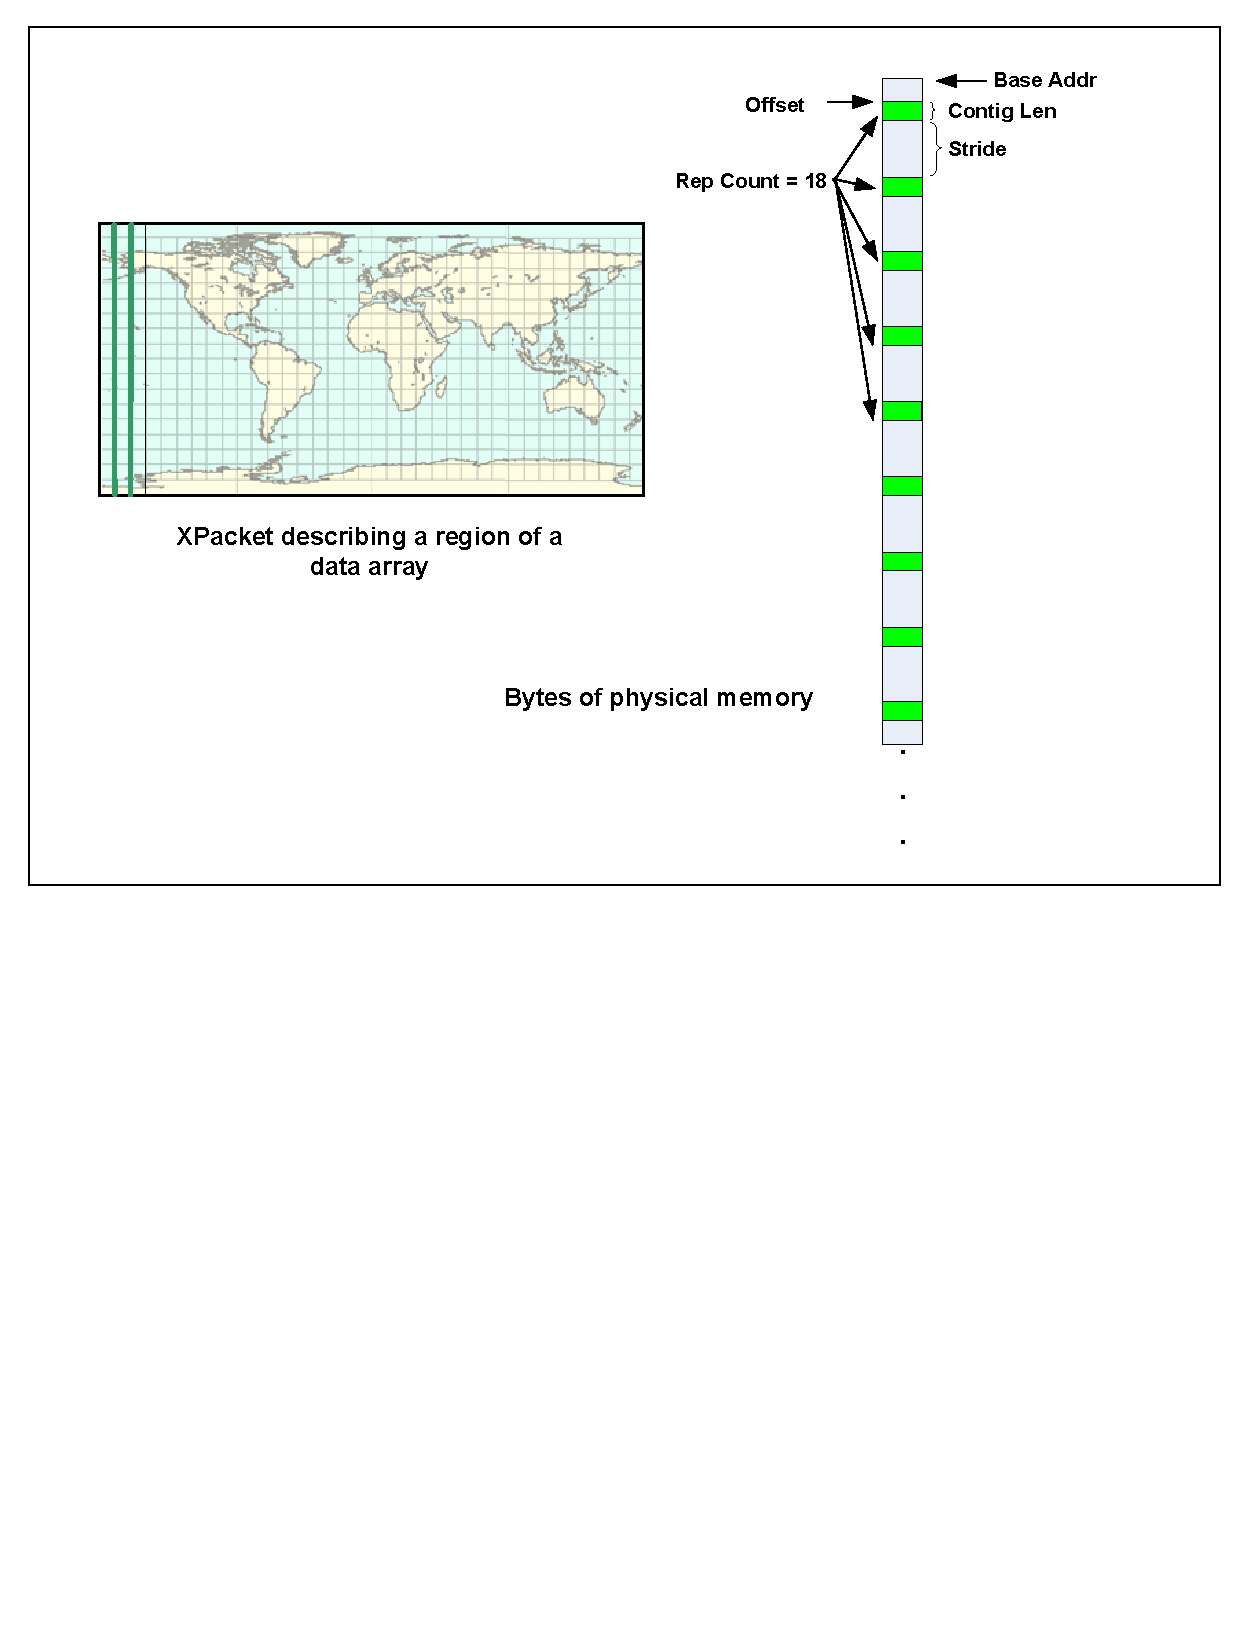
\includegraphics{Basic_xpacket_pack}}
\caption{A common XPacket pattern which generally benefits from
packing; the overlap region between 2 DEs during a halo update
are often short in the contiguous dimension and have a high 
repeat count.}
\label{fig:xpacketpack}
\end{figure}
\end{center}

\begin{center}
\begin{figure}
\scalebox{0.9}{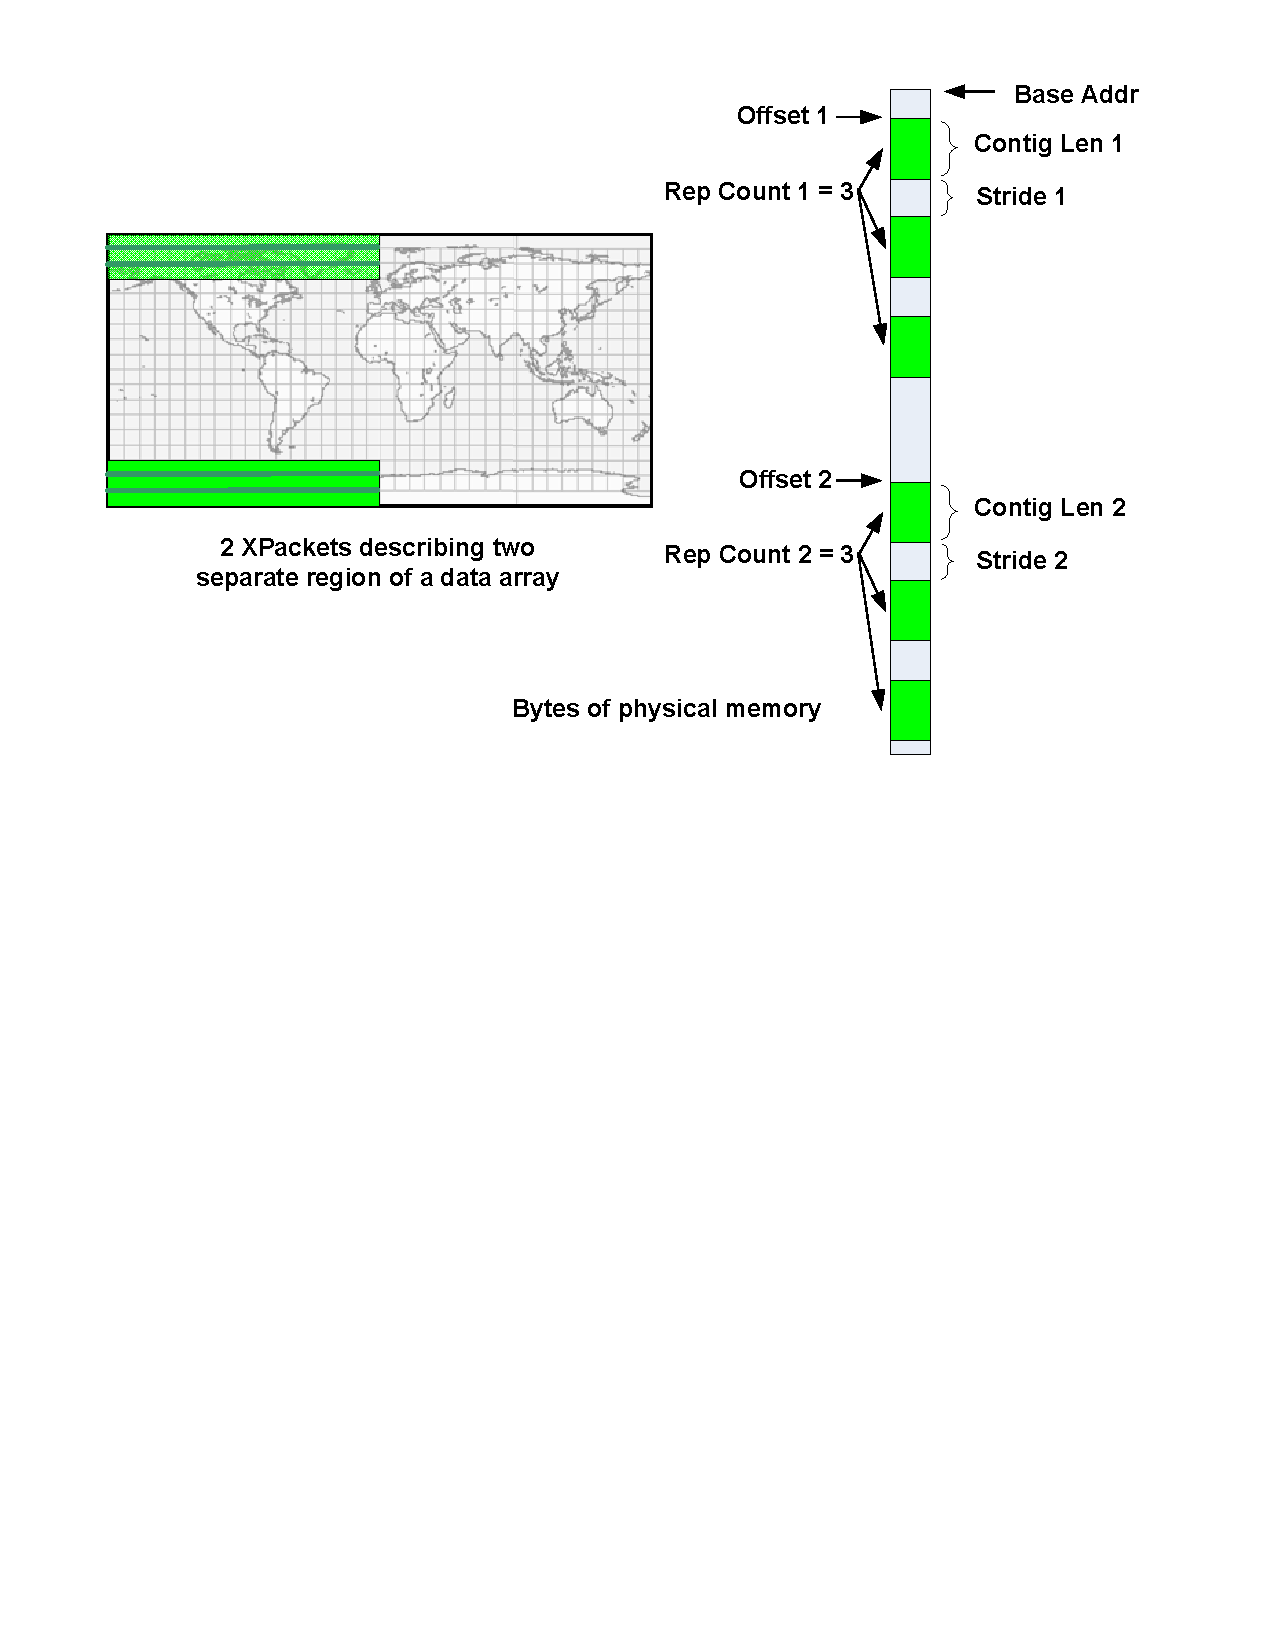
\includegraphics{Basic_xpacket_2up}}
\caption{When there are multiple XPackets destined for the
same remote PET there are more options for how to order the
contiguous pieces into a packed buffer.}
\label{fig:xpacket2up}
\end{figure}
\end{center}

\begin{center}
\begin{figure}
\caption{When the XPacket describes memory which is physically
a single contiguous region, there is no need to copy the data
into another buffer; it can be communicated inplace.  There is
a flag in the XPacket which marks how many of the dimensions
are contiguous.}
\label{fig:xpacketcontig}
\scalebox{0.9}{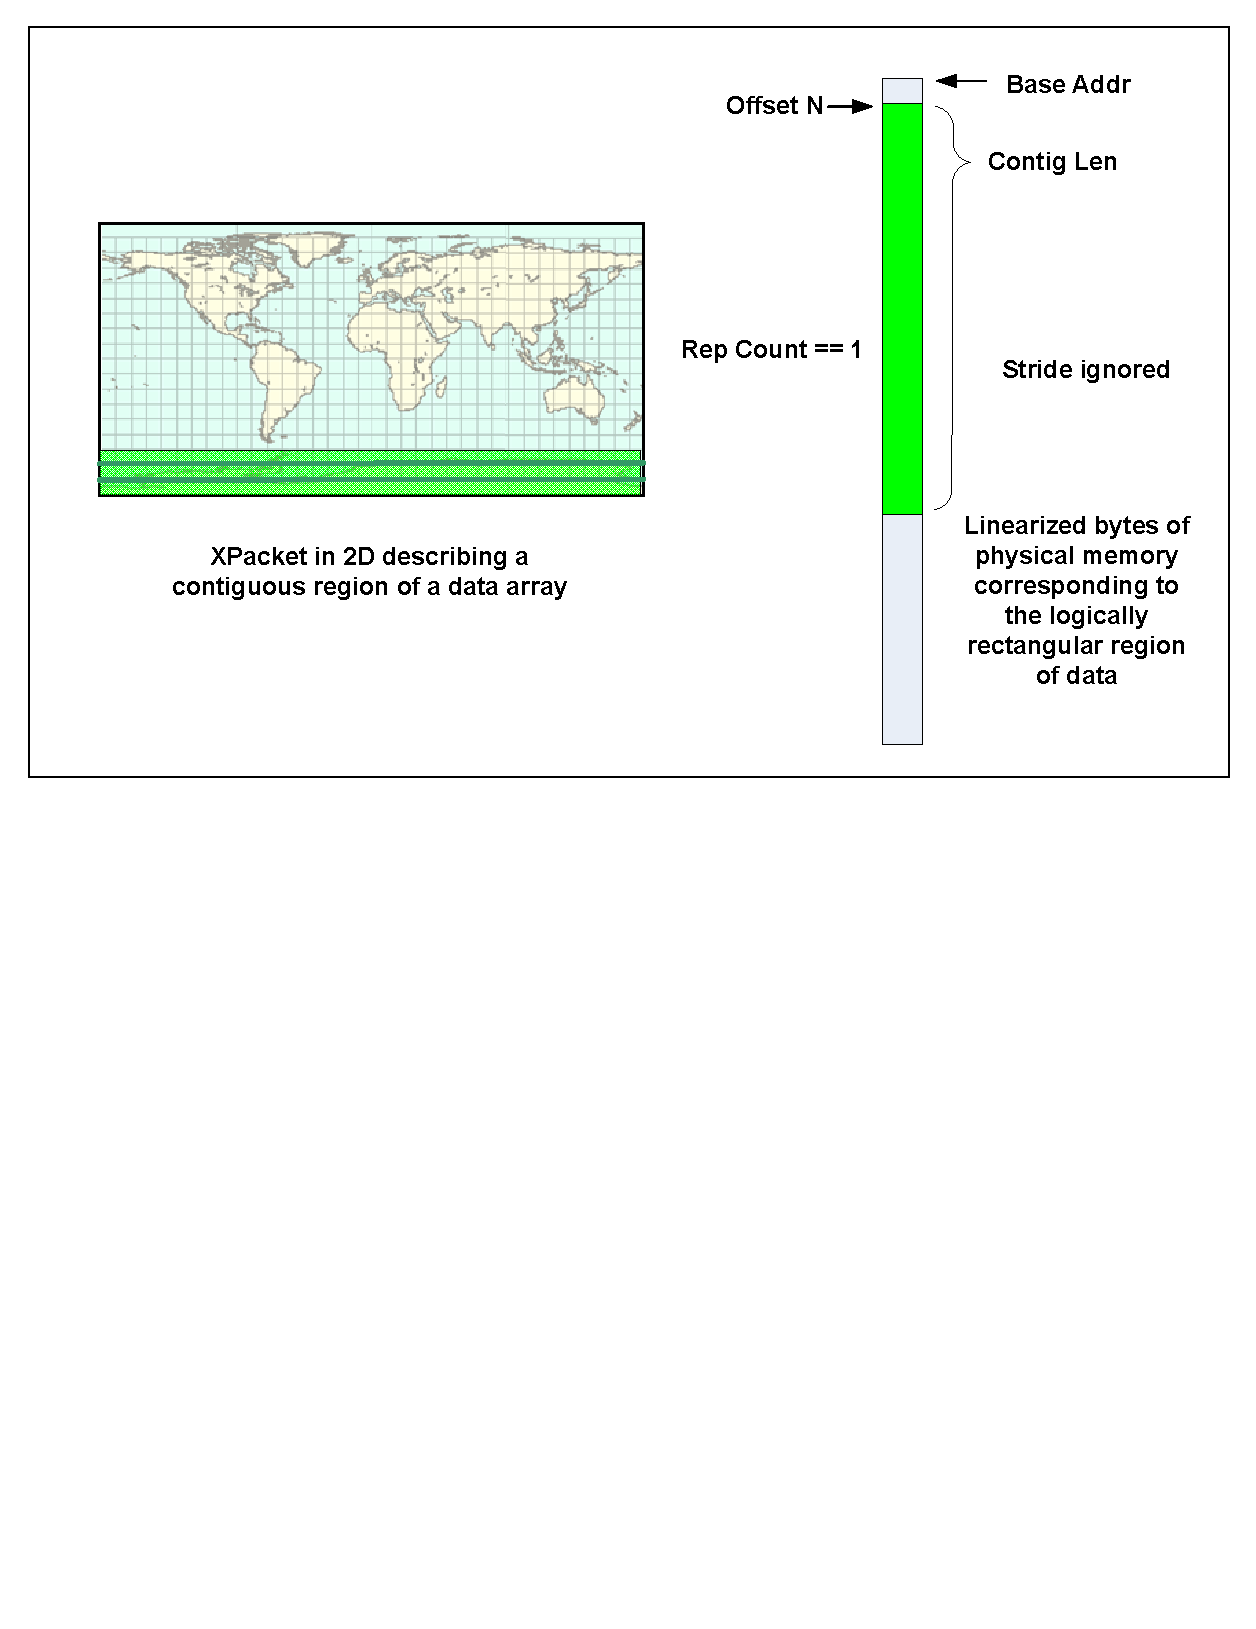
\includegraphics{Basic_xpacket_contig}}
\end{figure}
\end{center}

\begin{center}
\begin{figure}
\scalebox{0.9}{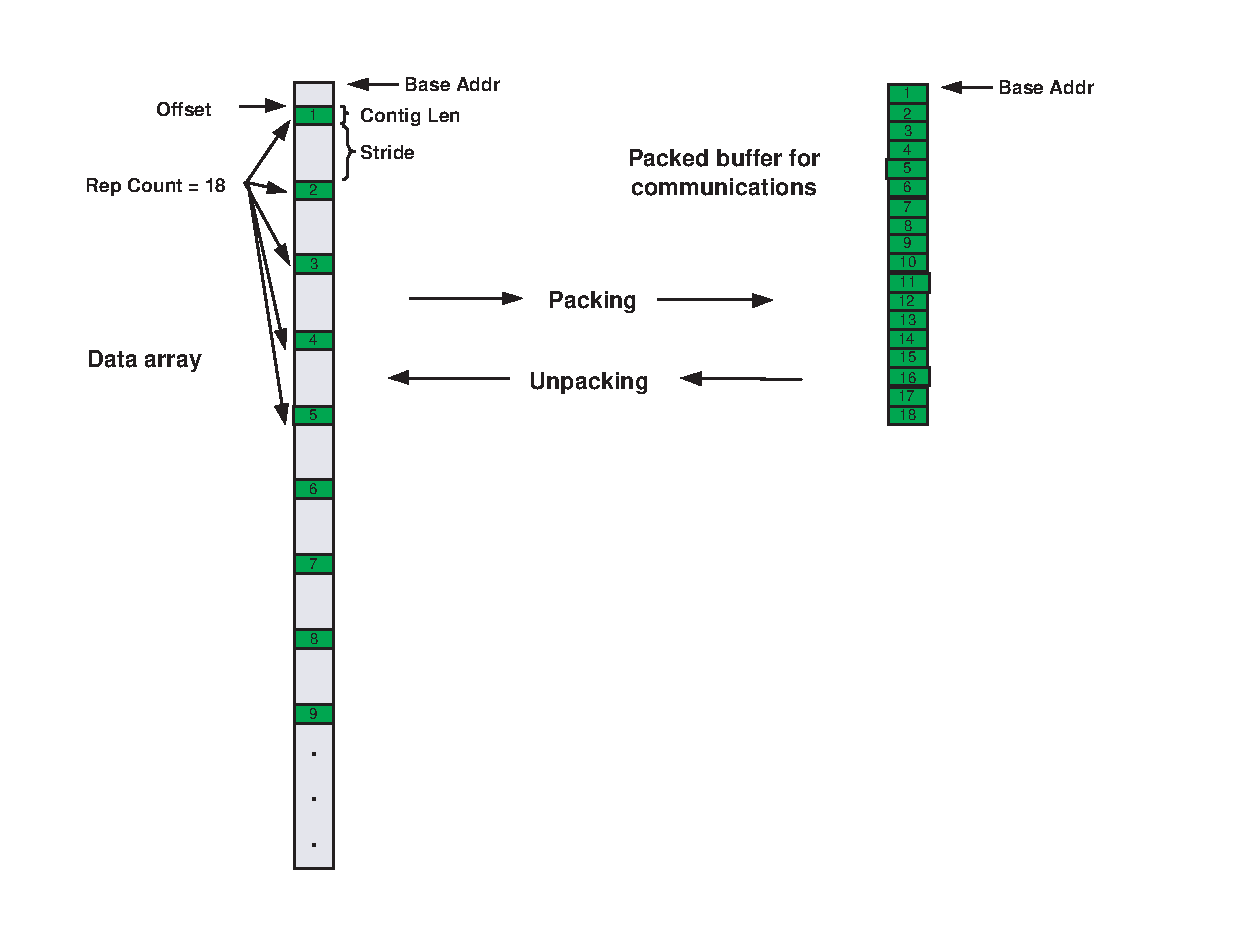
\includegraphics{Basic_pack_route}}
\caption{Often the overhead of making multiple communication calls 
outweighs the cost of copying non-contiguous data into a contiguous buffer,
sending it in a single operation, and then copying it to the final
memory locations on the receiving side.}
\label{fig:routepack}
\end{figure}
\end{center}

\begin{center}
\begin{figure}
\scalebox{0.9}{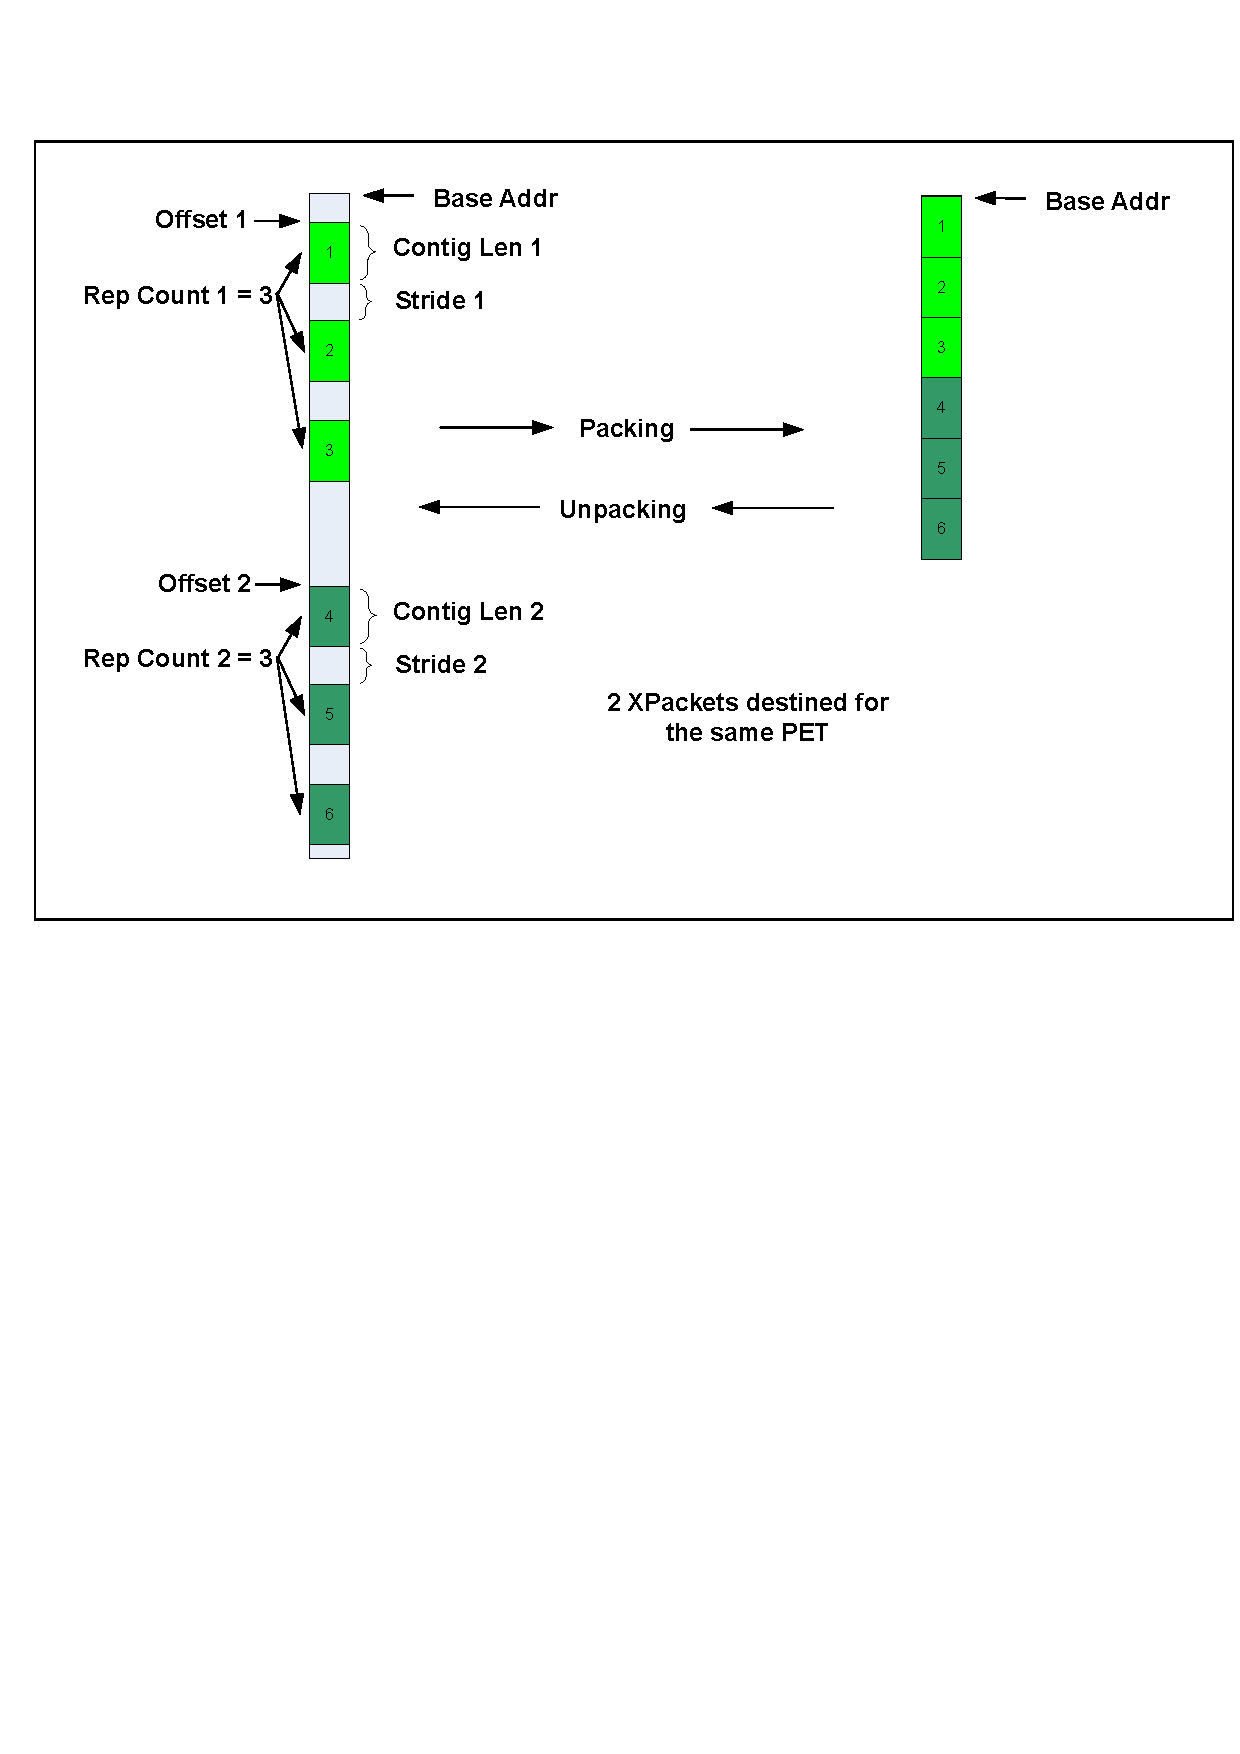
\includegraphics{Basic_2up_route}}
\caption{Once there is more than a single XPacket to pack, there
are many more interleave options.  For example, packing in the
order: 1, 4, 2, 5, 3, 6 would also be possible here.  However
the code becomes more complicated when the XPackets have different
repeat counts, and has no real performance advantage over the
straightforward packing of each XPacket in sequence.  Note that
this packing is the same whether it refers to multiple XPackets
from the same memory buffer or from multiple buffers.}
\label{fig:routepackall}
\end{figure}
\end{center}

The following options refer to the internal strategy for 
executing the route and not to whether the user-level API call
returns before the route has finished executing.  The current
system only implements user-synchronous calls; asynchronous calls
are on the to-be-written list.

\begin{enumerate}

\item[Sync] Each pair of processors exchanges data with the VM
equivalent of an MPI\_SendRecv() call, which does not return until
both the send and receive have completed.

\item[Async] Each processor executes both an asynchronous send
and asychronous receive to the other processor and does not wait
for completion before moving on to the next communication in the
CommTable.  Then in a separate loop through the RTables, each
call is waited for in turn and when all outstanding communication
calls have completed, then the API call returns to the user.

\end{enumerate}
(Note that in the Async case it makes much more sense to iterate
throught the Route table in PET order instead of the complication
of computing communication pairs and iterating in a non-sequential
order.  The code is as it is now for reasons of implementation speed
and not for any other design reason.  This would require a slightly
simpler, but separate, version of the RouteRun() subroutine.)

\item

FieldBundle-level communication calls have additional packing options
under certain circumstances.  FieldBundles are groups of Fields which
share the same Grid, but they are not required to share the same
data types, data ranks, nor relative data locations.  FieldBundles
in which these things are the same in all Fields are marked inside the
bundle code as being {\bf congruent}.  At communication store time
FieldBundles which have congruent data in all the Fields have the option
of packing all Field data together into fewer communication calls
which generally is expected to give better performance.   
Fields where the data is not of the same type or perhaps not
the same number of items (e.g. different rank, vertex-centered data
vs. cell centered data) can in theory also be packed but in fact
the code becomes more complicated, and in the case of differing
data types may cause system errors because of accessing data
on non-standard byte offsets or putting mixing integer data
with floating data and causing NaN (not a number) exceptions.
In this case, the conservative implementation strategy is to construct 
a separate Route object for each Field, all enclosed in the same
RouteHandle.  Inside the FieldBundle communication code the execution
for both types of FieldBundles is identical for the caller, but inside
the congruent FieldBundle code calls the {\tt ESMF\_RouteRun()} code
once and all communication for all Fields in the FieldBundle is done
when it returns.  The non-congruent FieldBundles execute a separate
{\tt ESMF\_RouteRun()} call for each Field and return to the user 
when all Field data have been sent/received.

There are comments in the code for an intermediate level of
optimization in which the FieldBundle code determines the smallest
number of unique types of Fields in the FieldBundle, and all same types
share the same Route object, but this has not been implemented
at this time.  Once the existing code has been in use for a while,
whether this is useful or needed may become more clear.


\item

The precompute code for all operations must have enough
information to compute which parts of the data arrays
are expected to be sent to remote PETs and also what
remote data is expected to be received by this PET.

These computations depend heavily on what type of distributed
method is being executed.  The regridding methods are described
in detail separately in the Regrid Design and Implementation Notes
section.  The halo and redistribution operations are described here.

\begin{enumerate}

\item[Halo] The total array area, which includes any halo regions,
are intersected with the computational
area of other DEs. The overlap regions are converted from index
space into memory space and stored as XPackets in the RTables.
This code must be aware of: whether the grid was defined as
periodic in any or all of the dimensions since that affects
which halo regions overlap at the grid edges; if the data
is only decomposed into a single block in any dimension (which
means it halos with itself); and if the halo region is large
enough that a halo operation may require intersection with
the N+1 neighbor in any dimension.  

\item[Redistribute]  Each DE computes the overlap
between its own computational region and all DEs in the 
remote Grid, again only working in computational area.  
The overlap regions are converted from index
space into memory space and stored as XPackets in the RTables.
After execution a redistribution, a halo operation may be required
to populate any halo regions with consistent data.

\end{enumerate}
(Note: the Redistribution code has been reimplemented to intersect
the DEs in index space and then convert the overlap region to an XPacket
representation.  Halo still converts the regions from AxisIndex to 
XPackets and then intersects the XPackets, but this code needs to be
changed to intersect in AxisIndex space and once the overlap is computed
then convert to XPackets.  Intersecting AxisIndex objects is very 
much simpler, both to understand and to execute, and more easily 
extensible to multiple dimensions than intersecting XPackets.)

\end{enumerate}

\subsection{Object Model}

The following is a simplified UML diagram showing the structure of the public
RouteHandle class.  See Appendix A, {\it A Brief Introduction to UML}, for a
translation table that lists the symbols in the diagram and their meaning.

\begin{center}
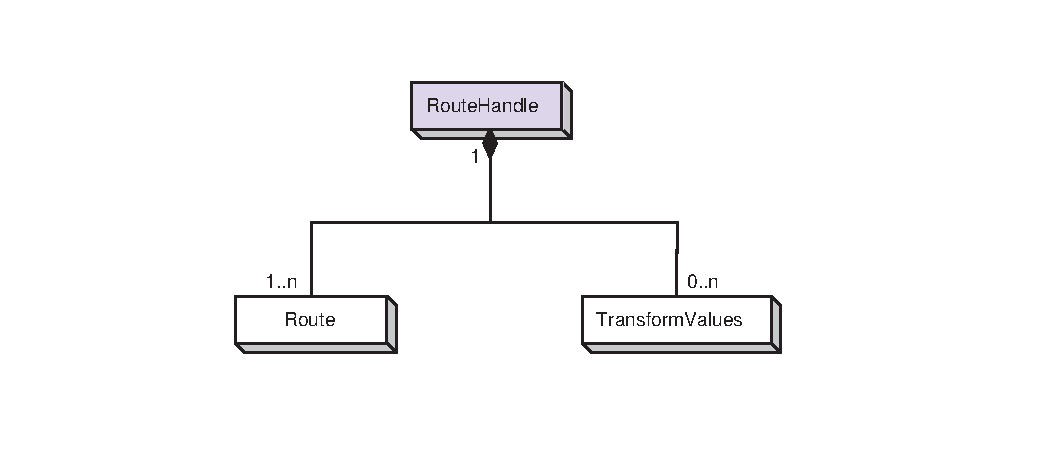
\includegraphics{RouteHandle_obj}
\end{center}


\subsection{File Based Regrid Weight Applications}
\label{sec:regrid:offline}

\subsubsection{Structured Grid to Structured Grid}

 In addition to the online regridding functionality, the ESMF distribution also 
contains an exectuable for generating regridding weights. This tool reads in
two grid files (in netcdf format) and outputs weights for interpolation
between the two grids.  The interpolation weights can be generated with either the bilinear
or patch method, both are described below, and there are also conservative regridding 
and pole handling options available.
This application assumes that the source and destination grids
are spherical and that the coordinates given in the files are latitude and longitude
values. This file based regrid weight generation application is fully parallel.

 To generate the interpolation weights, this tool first constructs two ESMF\_Mesh 
structures, one for the source and one for the destination grid. 
The coordinates for the Meshes are three dimensional, and are generated by mapping 
the latitudes and longitudes in the input grid files to 
3D Cartesian coordinates. The regridding occurs in 3D to avoid
problems with periodicity and with the pole singularity. To achieve periodicity 
the Meshes are constructed so that their left and right boundaries are connected. 
Unless the pole option is turned off, the polar region is handled by constructing 
an artificial point in the center of the top and bottom row of grid points. 
The pole is located at the average of the position of the points surrounding
it, but moved in the z-direction to be at the same radius as the rest of the points
in the grid. There are a couple of options for what value is used at the pole. 
The default is for the value at the pole to be the average of the values
of all of the grid points surrounding the pole. For another option, the user may also choose
a number N from 1 to the number of source grid points around the pole. For
each destination point, the value at the pole is then the average of the N source points
surrounding that destination point.

 This regridding application can be used to generate either bilinear or patch interpolation weights. The default interpolation method
is bilinear. The algorithm used by this application to generate the bilinear weights is the standard one found in
many textbooks.  Each destination point is mapped to a source cell, the position of the destination point relative to the cell's 
corners is used to calculate the interpolation weights. 

 This application can also be used to generate patch interpolation weights. Patch
interpolation is the ESMF version of a techique called ``patch recovery'' commonly
used in finite element modeling~\cite{PatchInterp1}~\cite{PatchInterp2}. It typically results in better approximations to values and derivatives when compared to bilinear interpolation.  
Patch interpolation works by constructing multiple polynomial patches to represent
the data in a source element. For 2D grids, these polynomials 
are currently 2nd degree 2D polynomials. The interpolated value at the destination point 
is the weighted average of the values of the patches at that point. 

The patch interpolation process works as follows. 
For each source element containing a destination point
we construct a patch for each corner node that makes up the element (e.g. 4 patches for 
quadrilateral elements, 3 for triangular elements). To construct a polynomial patch for
 a corner node we gather all the elements around that node. 
(Note that this means that the patch interpolation weights depends on the source 
element's nodes, and the nodes of all elements neighboring the source element.)  
We then use a least squares fitting algorithm to choose the set of coefficients 
for the polynomial that produces the best fit for the data in the elements. 
This polynomial will give a value at the destination point that fits the source data 
in the elements surrounding the corner node. We then repeat this process for each 
corner node of the source element generating a new polynomial for each set of elements.  
To calculate the value at the destination point we do a weighted average of the values 
of each of the corner polynomials evaluated at that point. The weight for a corner's 
polynomial is the bilinear weight of the destination point with regard to that corner.  

Global first-order conservative interpolation weights are also available with the 
file based regrid application. When this option is selected a conservative modification
is applied to the interpolation weights using the L2 method.  The L2 method in ESMF is based
on a finite element method to constrain the interpolation for global conservation of 
mass.  The conservative option can be used with either the patch or bilinear interpolation
and any of the pole options.  If this option is selected, integration weights will be
written to the output file containing the interpolation weights. 
Note that conservation is still in beta and should only be used with extreme caution.
It can have interpolation problems with certain combinations of source and destination grid. 
Particularly those where a high resolution area in the destination aligns with a lower resolution 
region in the source. 

The file based weight generation tool is located in src/Infrastructure/Mesh/examples 
directory and is called {\tt ESMC\_RegridWgtGenEx}. To use this tool ESMF must be compiled 
with the PNETCDF third party library. If the user wishes to use patch interpolation, 
then ESMF must additionally be compiled with the LAPACK third party library. Please see the 
``Third Party Libraries'' section of the ESMF User Guide for more information on this. 
The format for using the executable is as follows:

\begin{verbatim}

ESMC_RegridWgtGenEx [-conservative C] [-method M] [-pole P] <src> <dst> <weights>

Where:

 -conservative - An optional flag for indicating whether the interpolation weights should
                 be generated using the L2 conservation correction to the interpolation
                 method.  If this option is not specified it will default to "off".  The 
                 value C indicates the option that is given for this flag, C can have 
                 the following values:

                 off - Conservative correction is turned off. 
                 on  - Conservative correction is turned on.  

 -method       - An optional flag for indicating which interpolation method will be used.
                 If this option is not specified, then it will default to "bilinear".
                 The value M indicates which option is desired and it can have these 
                 values:

                 bilinear - This option selects the standard bilinear interpolation, this
                            is also the default option.
                 patch    - This option selects the ESMF version of patch recovery 
                            interpolation.

 -pole         - An optional flag for indicating what to do at the pole. If not 
                 specified, the pole defaults to option ``all'' described below. The 
                 value P indicates what should happen at the pole. P can have these 
                 values:

                 none - No pole, the source grid ends at the top (and bottom) row of 
                        nodes specified in <source grid>.
                 all  - Construct an artificial pole placed in the center of the 
                        top (or bottom) row of nodes, but projected onto the sphere 
                        formed by the rest of the grid. The value at this pole is the 
                        average of all the pole values.
                 <N>  - Construct an artificial pole placed in the center of the 
                        top (or bottom) row of nodes, but projected onto the sphere 
                        formed by the rest of the grid. The value at this pole is the 
                        average of the N source nodes next to the pole and surrounding
                        the destination point (i.e. the value may differ for each
                        destination point. Here N ranges from 1 to the number of nodes 
                        around the pole. 
                  
 <src>         - The netcdf file which holds the source grid for the interpolation. 
 
 <dst>         - The netcdf file which holds the destination grid for the interpolation. 

 <weights>     - The netcdf file which will contain the patch interpolation weights 
                 generated by the program.

\end{verbatim}

\subsubsection{Cubed Sphere to Structured Grid}

 In addition to the structured grid offline regridding functionality, the ESMF distribution also 
contains an exectuable for generating regridding weights between a cubed sphere grid and
a structured grid. This tool reads in
two grid files (in netcdf format) and outputs weights for interpolation
between the two grids.  The interpolation weights can be generated with either the bilinear, patch, or
conservative regridding. This application assumes that the source and destination grids
are spherical and that the coordinates given in the files are latitude and longitude
values. This file based regrid weight generation application generates the interpolation weights
in parallel.

 To generate the interpolation weights, this tool first constructs two ESMF\_Mesh 
structures, one for the source and one for the destination grid. 
The coordinates for the Meshes are three dimensional, and are generated by mapping 
the latitudes and longitudes in the input grid files to 
3D Cartesian coordinates. The regridding occurs in 3D to avoid
problems with the pole singularity. The cubed sphere grid is converted directly to 
a Mesh as is, but to achieve periodicity and to handle the pole, the structured grid
has some connectivity added. For the structured grid, the mesh is constructed so that 
it's left and right boundaries are connected. The polar region is handled by constructing 
an artificial point in the center of the top and bottom row of grid points. 
The pole is located at the average of the position of the points surrounding
it, but moved in the z-direction to be at the same radius as the rest of the points
in the grid. The value at the pole to be the average of the values
of all of the grid points surrounding the pole. 

 This regridding application can be used to generate bilinear, patch or conservative interpolation weights. The 
algorithm used by this application to generate the bilinear weights is the standard one found in
many textbooks.  Each destination point is mapped to a source cell, the position of the destination point relative 
to the cell's corners is used to calculate the interpolation weights. 

 This application can also be used to generate patch interpolation weights. Patch
interpolation is the ESMF version of a techique called ``patch recovery'' commonly
used in finite element modeling~\cite{PatchInterp1}~\cite{PatchInterp2}. It typically results in better approximations to values and derivatives when compared to bilinear interpolation.  
Patch interpolation works by constructing multiple polynomial patches to represent
the data in a source element. For 2D grids, these polynomials 
are currently 2nd degree 2D polynomials. The interpolated value at the destination point 
is the weighted average of the values of the patches at that point. 

The patch interpolation process works as follows. 
For each source element containing a destination point
we construct a patch for each corner node that makes up the element (e.g. 4 patches for 
quadrilateral elements, 3 for triangular elements). To construct a polynomial patch for
 a corner node we gather all the elements around that node. 
(Note that this means that the patch interpolation weights depends on the source 
element's nodes, and the nodes of all elements neighboring the source element.)  
We then use a least squares fitting algorithm to choose the set of coefficients 
for the polynomial that produces the best fit for the data in the elements. 
This polynomial will give a value at the destination point that fits the source data 
in the elements surrounding the corner node. We then repeat this process for each 
corner node of the source element generating a new polynomial for each set of elements.  
To calculate the value at the destination point we do a weighted average of the values 
of each of the corner polynomials evaluated at that point. The weight for a corner's 
polynomial is the bilinear weight of the destination point with regard to that corner.  

Global first-order conservative interpolation weights are also available with the 
file based regrid application. When this option is selected a conservative modification
is applied to bilinear interpolation weights using the L2 method.  The L2 method in ESMF is based
on a finite element method to constrain the interpolation for global conservation of 
mass. Note that this method is still in beta and should only be used with extreme caution.
It can have interpolation problems with certain combinations of source and destination grid. 
Particularly those where a high resolution area in the destination aligns with a lower resolution 
region in the source. 

The file based weight generation tool is located in src/Infrastructure/Mesh/examples 
directory and is called {\tt ESMF\_CubeSphereRegridEx}. To use this tool ESMF must be compiled 
with the NETCDF third party library. If the user wishes to use patch interpolation, 
then ESMF must additionally be compiled with the LAPACK third party library. Please see the 
``Third Party Libraries'' section of the ESMF User Guide for more information on this. 
The format for using the executable is as follows:

\begin{verbatim}

ESMF_CubeSphereRegridEx <cubed_grid> <struct_grid> <weights> method [rev]

Where:
                  
 <cubed_grid>  - The netcdf file which holds the cubed sphere grid for the interpolation. 
 
 <struct_grid> - The netcdf file which holds the structured grid for the interpolation. 

 <weights>     - The netcdf file which will contain the patch interpolation weights 
                 generated by the program.

  method       - A flag for indicating which interpolation method will be used.
                 The flag can have one of these values:

                 bilinear     - This option selects the standard bilinear interpolation.
                 patch        - This option selects the ESMF version of patch recovery 
                                interpolation.
                 conservative - This option selects conservative interpolation. 

  rev          - An optional flag that indicates the direction of the regridding. If not 
                 specified the <cubed_grid> is the source and the <struct_grid> is the 
                 destination. If 'rev' is specified, then the reverse interpolation is 
                 performed. 


\end{verbatim}




\newpage





